\documentclass[11pt]{article}
\usepackage[letterpaper,margin=0.8in,top=0.7in,bottom=0.8in]{geometry}
\usepackage[T1]{fontenc}
\usepackage[scaled]{helvet}
\renewcommand{\familydefault}{\sfdefault}
\usepackage{amsmath,amssymb}
\usepackage[table]{xcolor}
\usepackage[most]{tcolorbox}
\usepackage{multicol}
\usepackage{needspace}
\usepackage{fancyhdr}
\usepackage{enumitem}

% Palette F. Bright & Playful
\definecolor{fmtitle}{HTML}{3D2C8D}
\definecolor{fmkey}{HTML}{0096C7}
\definecolor{fmwatch}{HTML}{2BB673}
\definecolor{fmturn}{HTML}{F4A100}
\definecolor{fmans}{HTML}{EF476F}
\definecolor{fmnotice}{HTML}{9B5DE5}
\definecolor{fmgray}{HTML}{555555}

\pagestyle{fancy}\fancyhf{}
\renewcommand{\headrulewidth}{0pt}
\fancyfoot[L]{\small\color{fmgray}\textcopyright\ 2026 FangMath. All rights reserved.}
\fancyfoot[R]{\small\color{fmgray}\thepage}
\setlength{\parindent}{0pt}

\newtcolorbox{keyidea}{enhanced,colback=fmkey!7,colframe=fmkey,boxrule=0.9pt,arc=2mm,
  title={Key Idea},fonttitle=\bfseries,coltitle=fmkey,
  attach boxed title to top left={xshift=4mm,yshift=-2mm},
  boxed title style={colback=white,colframe=fmkey,boxrule=0.9pt},top=4mm}
\newtcolorbox{watchme}{enhanced,colback=fmwatch!7,colframe=fmwatch,boxrule=0.9pt,arc=2mm,
  title={Watch Me},fonttitle=\bfseries,coltitle=fmwatch,
  attach boxed title to top left={xshift=4mm,yshift=-2mm},
  boxed title style={colback=white,colframe=fmwatch,boxrule=0.9pt},top=4mm}
\newtcolorbox{mistake}{enhanced,colback=fmans!6,colframe=fmans,boxrule=0.9pt,arc=2mm,
  title={Common Mistake},fonttitle=\bfseries,coltitle=fmans,
  attach boxed title to top left={xshift=4mm,yshift=-2mm},
  boxed title style={colback=white,colframe=fmans,boxrule=0.9pt},top=4mm}
\newtcolorbox{challenge}{enhanced,colback=fmnotice!6,colframe=fmnotice,boxrule=0.9pt,arc=2mm,
  title={Challenge},fonttitle=\bfseries,coltitle=fmnotice,
  attach boxed title to top left={xshift=4mm,yshift=-2mm},
  boxed title style={colback=white,colframe=fmnotice,boxrule=0.9pt},top=4mm}

\newcommand{\badge}[1]{\colorbox{fmtitle}{\color{white}\bfseries\small\,#1\,}}
\newcommand{\parttitle}[2]{\needspace{6cm}\vspace{4mm}%
  {\colorbox{fmtitle}{\parbox{\dimexpr\linewidth-2\fboxsep}{\color{white}\bfseries\large Part #1 \quad #2}}}\par\vspace{3mm}}
\newcommand{\blank}{\underline{\hspace{2.2cm}}}
\newcommand{\sblank}{\underline{\hspace{1.3cm}}}
\newcommand{\ans}[1]{\textcolor{fmans}{\textbf{#1}}}
\usepackage{tikz}
\newcommand{\leveltag}[2]{\colorbox{#1}{\color{white}\bfseries\small\,#2\,}}
\newcommand{\bk}{\underline{\hspace{0.9cm}}}
\newcommand{\lbk}{\underline{\hspace{1.6cm}}}

\begin{document}
\badge{PRACTICE SET}\hfill{\color{fmgray}\small FangMath}\par\vspace{3mm}
{\color{fmtitle}\bfseries\LARGE Getting Ready for Similarity}\par\vspace{1mm}
{\color{fmgray}\large Similar rectangles and similar triangles}\par\vspace{4mm}
Name: \underline{\hspace{6cm}} \hfill Date: \underline{\hspace{3.5cm}}\par\vspace{2mm}

\parttitle{A}{Similar Rectangles}
\begin{keyidea}
Two shapes are \textbf{similar} when one is an enlargement (or shrink) of the other: \textbf{same shape, different size}.
For rectangles, \textbf{long side $\leftrightarrow$ long side} and \textbf{short side $\leftrightarrow$ short side}. The rectangles are similar when both ratios are the same number:
\[ \frac{\text{long side of 2nd}}{\text{long side of 1st}} \;=\; \frac{\text{short side of 2nd}}{\text{short side of 1st}} \;=\; \text{scale factor} \]
\end{keyidea}
\begin{watchme}\textbf{Example 1 --- Are they similar?}\par\vspace{2mm}\begin{minipage}[c]{0.42\linewidth}\centering 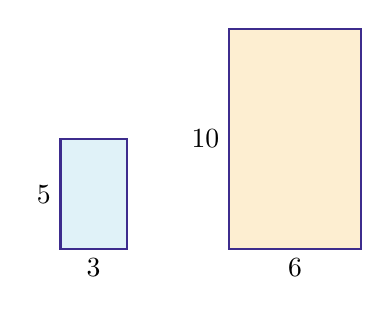
\begin{tikzpicture}[baseline=0pt]\filldraw[fill=fmkey!12,draw=fmtitle,thick] (0,0) rectangle (0.840,1.400);\node[below] at (0.420,0) {$3$};\node[left] at (0,0.700) {$5$};\filldraw[fill=fmturn!18,draw=fmtitle,thick] (2.140,0) rectangle (3.820,2.800);\node[below] at (2.980,0) {$6$};\node[left] at (2.140,1.400) {$10$};\end{tikzpicture}\end{minipage}\hfill\begin{minipage}[c]{0.55\linewidth}Long sides: $\dfrac{10}{5} = 2$ \qquad Short sides: $\dfrac{6}{3} = 2$\par\vspace{1mm}Both ratios are $2$, so the rectangles \textbf{are similar}.\par Scale factor $=\mathbf{2}$.\end{minipage}\end{watchme}
\begin{watchme}\textbf{Example 2 --- Find the missing side.} \;The rectangles are similar.\par\vspace{2mm}\begin{minipage}[c]{0.42\linewidth}\centering 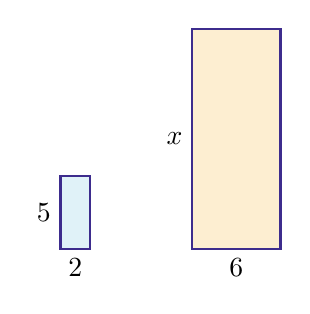
\begin{tikzpicture}[baseline=0pt]\filldraw[fill=fmkey!12,draw=fmtitle,thick] (0,0) rectangle (0.373,0.933);\node[below] at (0.187,0) {$2$};\node[left] at (0,0.467) {$5$};\filldraw[fill=fmturn!18,draw=fmtitle,thick] (1.673,0) rectangle (2.793,2.800);\node[below] at (2.233,0) {$6$};\node[left] at (1.673,1.400) {$x$};\end{tikzpicture}\end{minipage}\hfill\begin{minipage}[c]{0.55\linewidth}{\color{fmwatch}\textbf{Method 1 --- Scale factor}}\par\vspace{1.5mm} Use the pair you know: \;$\dfrac{6}{2} = 3$, so the scale factor is $3$.\par\vspace{1mm} Multiply: \;$x = 5 \times 3 = \mathbf{15}$.\par\vspace{2mm}{\color{fmwatch}\textbf{Method 2 --- Proportion}}\par\vspace{1.5mm} Write $\dfrac{\text{2nd}}{\text{1st}}$ for both pairs of matching sides:\par\vspace{1mm}$\dfrac{6}{2} = \dfrac{x}{5}$ \;$\Rightarrow$\; $2x = 6 \times 5 = 30$ \;$\Rightarrow$\; $x = \mathbf{15}$\end{minipage}\end{watchme}
\begin{mistake}
$2 \times 3$ and $4 \times 5$ are \textbf{not} similar. Adding $2$ to every side changes the shape.
Similar shapes come from \textbf{multiplying} every side by the same number.
\end{mistake}
\newpage
\leveltag{fmwatch}{EASY}\quad{\color{fmtitle}\bfseries Rectangles}\par\vspace{1mm}{\small Problems 1--5: Are the rectangles similar? If yes, give the scale factor (1st $\to$ 2nd). }\par\vspace{4mm}
\needspace{6.2cm}\noindent \begin{minipage}[t]{0.485\linewidth}\textbf{1.}\par\vspace{1mm}\centering 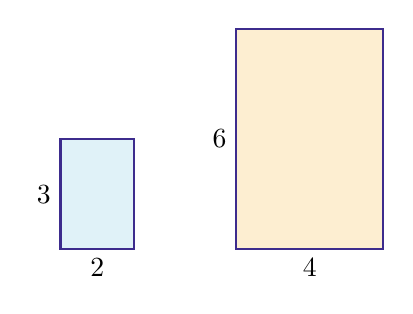
\begin{tikzpicture}[baseline=0pt]\filldraw[fill=fmkey!12,draw=fmtitle,thick] (0,0) rectangle (0.933,1.400);\node[below] at (0.467,0) {$2$};\node[left] at (0,0.700) {$3$};\filldraw[fill=fmturn!18,draw=fmtitle,thick] (2.233,0) rectangle (4.100,2.800);\node[below] at (3.167,0) {$4$};\node[left] at (2.233,1.400) {$6$};\end{tikzpicture}\par\vspace{3mm}\raggedright {\small Long sides: $\dfrac{\bk}{\bk}$ \quad Short sides: $\dfrac{\bk}{\bk}$}\par\vspace{1.5mm}{\small Similar? \; Yes \; / \; No \qquad Scale factor: \bk}\end{minipage}\hfill \begin{minipage}[t]{0.485\linewidth}\textbf{2.}\par\vspace{1mm}\centering 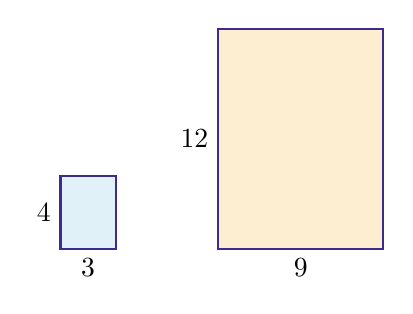
\begin{tikzpicture}[baseline=0pt]\filldraw[fill=fmkey!12,draw=fmtitle,thick] (0,0) rectangle (0.700,0.933);\node[below] at (0.350,0) {$3$};\node[left] at (0,0.467) {$4$};\filldraw[fill=fmturn!18,draw=fmtitle,thick] (2.000,0) rectangle (4.100,2.800);\node[below] at (3.050,0) {$9$};\node[left] at (2.000,1.400) {$12$};\end{tikzpicture}\par\vspace{3mm}\raggedright {\small Long sides: $\dfrac{\bk}{\bk}$ \quad Short sides: $\dfrac{\bk}{\bk}$}\par\vspace{1.5mm}{\small Similar? \; Yes \; / \; No \qquad Scale factor: \bk}\end{minipage}\par\vspace{12mm}
\needspace{6.2cm}\noindent \begin{minipage}[t]{0.485\linewidth}\textbf{3.}\par\vspace{1mm}\centering 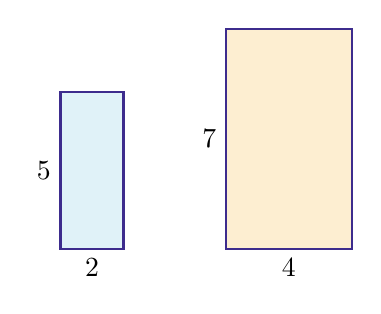
\begin{tikzpicture}[baseline=0pt]\filldraw[fill=fmkey!12,draw=fmtitle,thick] (0,0) rectangle (0.800,2.000);\node[below] at (0.400,0) {$2$};\node[left] at (0,1.000) {$5$};\filldraw[fill=fmturn!18,draw=fmtitle,thick] (2.100,0) rectangle (3.700,2.800);\node[below] at (2.900,0) {$4$};\node[left] at (2.100,1.400) {$7$};\end{tikzpicture}\par\vspace{3mm}\raggedright {\small Long sides: $\dfrac{\bk}{\bk}$ \quad Short sides: $\dfrac{\bk}{\bk}$}\par\vspace{1.5mm}{\small Similar? \; Yes \; / \; No \qquad Scale factor: \bk}\end{minipage}\hfill \begin{minipage}[t]{0.485\linewidth}\textbf{4.}\par\vspace{1mm}\centering 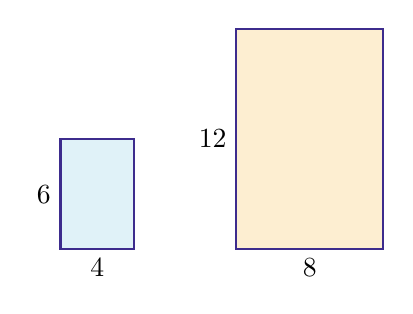
\begin{tikzpicture}[baseline=0pt]\filldraw[fill=fmkey!12,draw=fmtitle,thick] (0,0) rectangle (0.933,1.400);\node[below] at (0.467,0) {$4$};\node[left] at (0,0.700) {$6$};\filldraw[fill=fmturn!18,draw=fmtitle,thick] (2.233,0) rectangle (4.100,2.800);\node[below] at (3.167,0) {$8$};\node[left] at (2.233,1.400) {$12$};\end{tikzpicture}\par\vspace{3mm}\raggedright {\small Long sides: $\dfrac{\bk}{\bk}$ \quad Short sides: $\dfrac{\bk}{\bk}$}\par\vspace{1.5mm}{\small Similar? \; Yes \; / \; No \qquad Scale factor: \bk}\end{minipage}\par\vspace{12mm}
\needspace{6.2cm}\noindent \begin{minipage}[t]{0.485\linewidth}\textbf{5.}\par\vspace{1mm}\centering 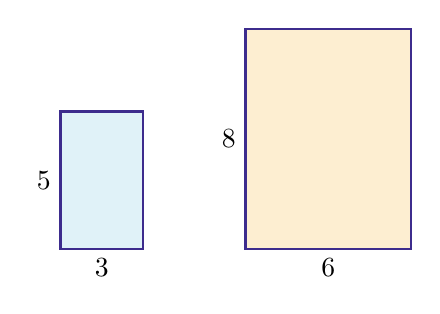
\begin{tikzpicture}[baseline=0pt]\filldraw[fill=fmkey!12,draw=fmtitle,thick] (0,0) rectangle (1.050,1.750);\node[below] at (0.525,0) {$3$};\node[left] at (0,0.875) {$5$};\filldraw[fill=fmturn!18,draw=fmtitle,thick] (2.350,0) rectangle (4.450,2.800);\node[below] at (3.400,0) {$6$};\node[left] at (2.350,1.400) {$8$};\end{tikzpicture}\par\vspace{3mm}\raggedright {\small Long sides: $\dfrac{\bk}{\bk}$ \quad Short sides: $\dfrac{\bk}{\bk}$}\par\vspace{1.5mm}{\small Similar? \; Yes \; / \; No \qquad Scale factor: \bk}\end{minipage}\par\vspace{12mm}
\newpage
\leveltag{fmwatch}{EASY}\quad{\color{fmtitle}\bfseries Rectangles --- Find the Missing Side}\par\vspace{1mm}{\small The rectangles are similar. Find $x$ two ways: with the scale factor and with a proportion.}\par\vspace{5mm}
\needspace{6.2cm}\noindent \begin{minipage}[t]{0.485\linewidth}\textbf{6.}\par\vspace{1mm}\centering 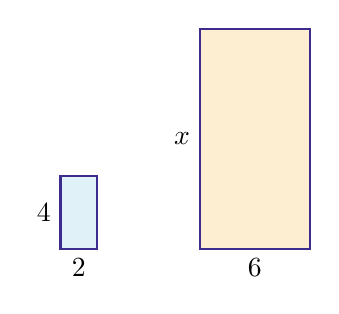
\begin{tikzpicture}[baseline=0pt]\filldraw[fill=fmkey!12,draw=fmtitle,thick] (0,0) rectangle (0.467,0.933);\node[below] at (0.233,0) {$2$};\node[left] at (0,0.467) {$4$};\filldraw[fill=fmturn!18,draw=fmtitle,thick] (1.767,0) rectangle (3.167,2.800);\node[below] at (2.467,0) {$6$};\node[left] at (1.767,1.400) {$x$};\end{tikzpicture}\par\vspace{3mm}\raggedright {\small\textbf{Method 1} --- Scale factor: \bk \quad $x = $ \bk}\par\vspace{2mm}{\small\textbf{Method 2} --- Proportion: $\dfrac{\bk}{\bk} = \dfrac{\bk}{\bk}$ \quad $x = $ \bk}\end{minipage}\hfill \begin{minipage}[t]{0.485\linewidth}\textbf{7.}\par\vspace{1mm}\centering 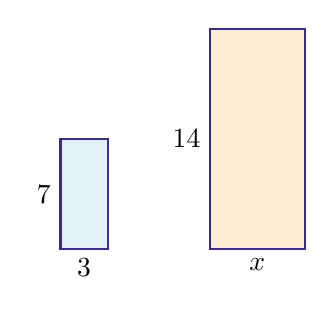
\begin{tikzpicture}[baseline=0pt]\filldraw[fill=fmkey!12,draw=fmtitle,thick] (0,0) rectangle (0.600,1.400);\node[below] at (0.300,0) {$3$};\node[left] at (0,0.700) {$7$};\filldraw[fill=fmturn!18,draw=fmtitle,thick] (1.900,0) rectangle (3.100,2.800);\node[below] at (2.500,0) {$x$};\node[left] at (1.900,1.400) {$14$};\end{tikzpicture}\par\vspace{3mm}\raggedright {\small\textbf{Method 1} --- Scale factor: \bk \quad $x = $ \bk}\par\vspace{2mm}{\small\textbf{Method 2} --- Proportion: $\dfrac{\bk}{\bk} = \dfrac{\bk}{\bk}$ \quad $x = $ \bk}\end{minipage}\par\vspace{14mm}
\needspace{6.2cm}\noindent \begin{minipage}[t]{0.485\linewidth}\textbf{8.}\par\vspace{1mm}\centering 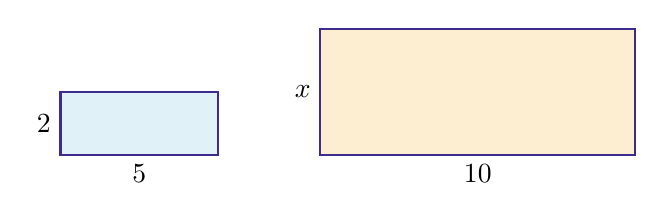
\begin{tikzpicture}[baseline=0pt]\filldraw[fill=fmkey!12,draw=fmtitle,thick] (0,0) rectangle (2.000,0.800);\node[below] at (1.000,0) {$5$};\node[left] at (0,0.400) {$2$};\filldraw[fill=fmturn!18,draw=fmtitle,thick] (3.300,0) rectangle (7.300,1.600);\node[below] at (5.300,0) {$10$};\node[left] at (3.300,0.800) {$x$};\end{tikzpicture}\par\vspace{3mm}\raggedright {\small\textbf{Method 1} --- Scale factor: \bk \quad $x = $ \bk}\par\vspace{2mm}{\small\textbf{Method 2} --- Proportion: $\dfrac{\bk}{\bk} = \dfrac{\bk}{\bk}$ \quad $x = $ \bk}\end{minipage}\hfill \begin{minipage}[t]{0.485\linewidth}\textbf{9.}\par\vspace{1mm}\centering 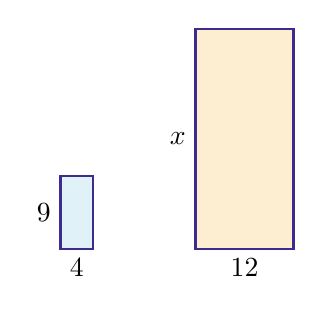
\begin{tikzpicture}[baseline=0pt]\filldraw[fill=fmkey!12,draw=fmtitle,thick] (0,0) rectangle (0.415,0.933);\node[below] at (0.207,0) {$4$};\node[left] at (0,0.467) {$9$};\filldraw[fill=fmturn!18,draw=fmtitle,thick] (1.715,0) rectangle (2.959,2.800);\node[below] at (2.337,0) {$12$};\node[left] at (1.715,1.400) {$x$};\end{tikzpicture}\par\vspace{3mm}\raggedright {\small\textbf{Method 1} --- Scale factor: \bk \quad $x = $ \bk}\par\vspace{2mm}{\small\textbf{Method 2} --- Proportion: $\dfrac{\bk}{\bk} = \dfrac{\bk}{\bk}$ \quad $x = $ \bk}\end{minipage}\par\vspace{14mm}
\needspace{6.2cm}\noindent \begin{minipage}[t]{0.485\linewidth}\textbf{10.}\par\vspace{1mm}\centering 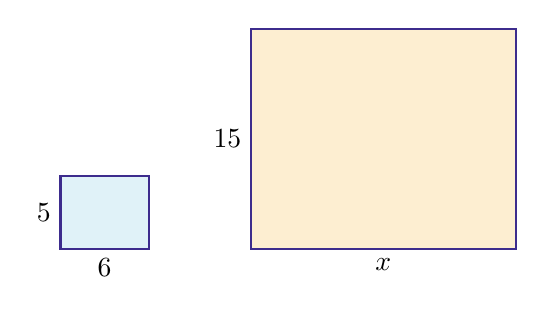
\begin{tikzpicture}[baseline=0pt]\filldraw[fill=fmkey!12,draw=fmtitle,thick] (0,0) rectangle (1.120,0.933);\node[below] at (0.560,0) {$6$};\node[left] at (0,0.467) {$5$};\filldraw[fill=fmturn!18,draw=fmtitle,thick] (2.420,0) rectangle (5.780,2.800);\node[below] at (4.100,0) {$x$};\node[left] at (2.420,1.400) {$15$};\end{tikzpicture}\par\vspace{3mm}\raggedright {\small\textbf{Method 1} --- Scale factor: \bk \quad $x = $ \bk}\par\vspace{2mm}{\small\textbf{Method 2} --- Proportion: $\dfrac{\bk}{\bk} = \dfrac{\bk}{\bk}$ \quad $x = $ \bk}\end{minipage}\par\vspace{14mm}
\newpage
\leveltag{fmturn}{MEDIUM}\quad{\color{fmtitle}\bfseries Rectangles}\par\vspace{1mm}{\small Problems 1--5: Are the rectangles similar? Watch out --- a rectangle may be turned sideways, and the scale factor may be a fraction.}\par\vspace{4mm}
\needspace{6.2cm}\noindent \begin{minipage}[t]{0.485\linewidth}\textbf{1.}\par\vspace{1mm}\centering 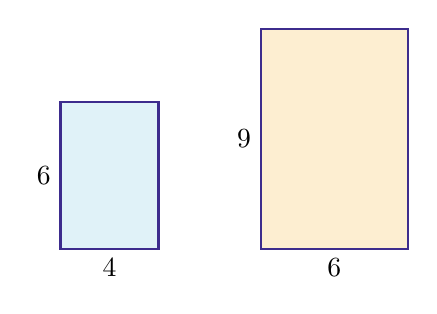
\begin{tikzpicture}[baseline=0pt]\filldraw[fill=fmkey!12,draw=fmtitle,thick] (0,0) rectangle (1.244,1.867);\node[below] at (0.622,0) {$4$};\node[left] at (0,0.933) {$6$};\filldraw[fill=fmturn!18,draw=fmtitle,thick] (2.544,0) rectangle (4.411,2.800);\node[below] at (3.478,0) {$6$};\node[left] at (2.544,1.400) {$9$};\end{tikzpicture}\par\vspace{3mm}\raggedright {\small Long sides: $\dfrac{\bk}{\bk}$ \quad Short sides: $\dfrac{\bk}{\bk}$}\par\vspace{1.5mm}{\small Similar? \; Yes \; / \; No \qquad Scale factor: \bk}\end{minipage}\hfill \begin{minipage}[t]{0.485\linewidth}\textbf{2.}\par\vspace{1mm}\centering 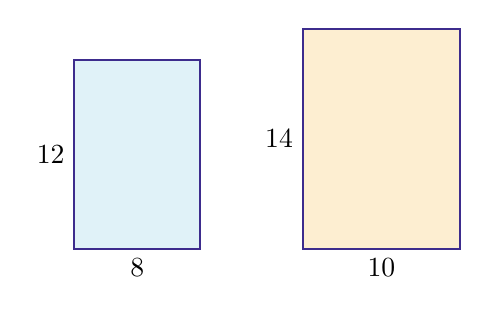
\begin{tikzpicture}[baseline=0pt]\filldraw[fill=fmkey!12,draw=fmtitle,thick] (0,0) rectangle (1.600,2.400);\node[below] at (0.800,0) {$8$};\node[left] at (0,1.200) {$12$};\filldraw[fill=fmturn!18,draw=fmtitle,thick] (2.900,0) rectangle (4.900,2.800);\node[below] at (3.900,0) {$10$};\node[left] at (2.900,1.400) {$14$};\end{tikzpicture}\par\vspace{3mm}\raggedright {\small Long sides: $\dfrac{\bk}{\bk}$ \quad Short sides: $\dfrac{\bk}{\bk}$}\par\vspace{1.5mm}{\small Similar? \; Yes \; / \; No \qquad Scale factor: \bk}\end{minipage}\par\vspace{12mm}
\needspace{6.2cm}\noindent \begin{minipage}[t]{0.485\linewidth}\textbf{3.}\par\vspace{1mm}\centering 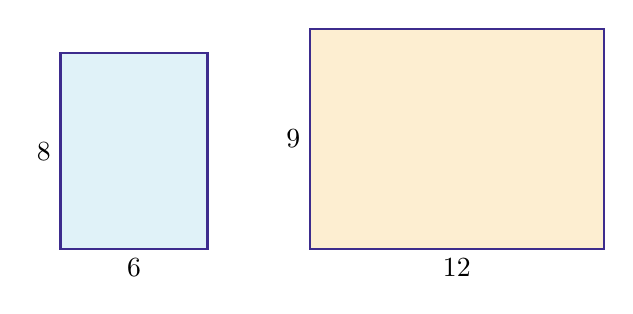
\begin{tikzpicture}[baseline=0pt]\filldraw[fill=fmkey!12,draw=fmtitle,thick] (0,0) rectangle (1.867,2.489);\node[below] at (0.933,0) {$6$};\node[left] at (0,1.244) {$8$};\filldraw[fill=fmturn!18,draw=fmtitle,thick] (3.167,0) rectangle (6.900,2.800);\node[below] at (5.033,0) {$12$};\node[left] at (3.167,1.400) {$9$};\end{tikzpicture}\par\vspace{3mm}\raggedright {\small Long sides: $\dfrac{\bk}{\bk}$ \quad Short sides: $\dfrac{\bk}{\bk}$}\par\vspace{1.5mm}{\small Similar? \; Yes \; / \; No \qquad Scale factor: \bk}\end{minipage}\hfill \begin{minipage}[t]{0.485\linewidth}\textbf{4.}\par\vspace{1mm}\centering 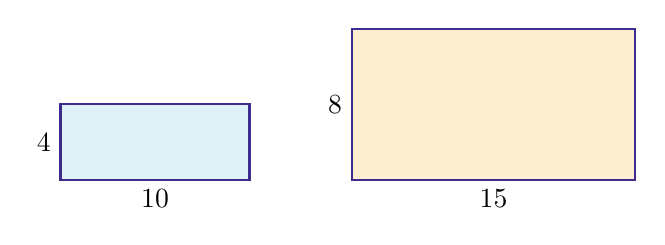
\begin{tikzpicture}[baseline=0pt]\filldraw[fill=fmkey!12,draw=fmtitle,thick] (0,0) rectangle (2.400,0.960);\node[below] at (1.200,0) {$10$};\node[left] at (0,0.480) {$4$};\filldraw[fill=fmturn!18,draw=fmtitle,thick] (3.700,0) rectangle (7.300,1.920);\node[below] at (5.500,0) {$15$};\node[left] at (3.700,0.960) {$8$};\end{tikzpicture}\par\vspace{3mm}\raggedright {\small Long sides: $\dfrac{\bk}{\bk}$ \quad Short sides: $\dfrac{\bk}{\bk}$}\par\vspace{1.5mm}{\small Similar? \; Yes \; / \; No \qquad Scale factor: \bk}\end{minipage}\par\vspace{12mm}
\needspace{6.2cm}\noindent \begin{minipage}[t]{0.485\linewidth}\textbf{5.}\par\vspace{1mm}\centering 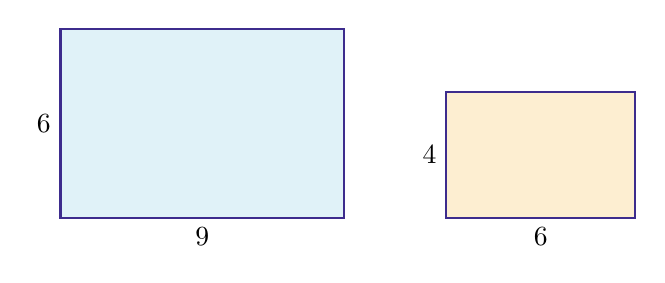
\begin{tikzpicture}[baseline=0pt]\filldraw[fill=fmkey!12,draw=fmtitle,thick] (0,0) rectangle (3.600,2.400);\node[below] at (1.800,0) {$9$};\node[left] at (0,1.200) {$6$};\filldraw[fill=fmturn!18,draw=fmtitle,thick] (4.900,0) rectangle (7.300,1.600);\node[below] at (6.100,0) {$6$};\node[left] at (4.900,0.800) {$4$};\end{tikzpicture}\par\vspace{3mm}\raggedright {\small Long sides: $\dfrac{\bk}{\bk}$ \quad Short sides: $\dfrac{\bk}{\bk}$}\par\vspace{1.5mm}{\small Similar? \; Yes \; / \; No \qquad Scale factor: \bk}\end{minipage}\par\vspace{12mm}
\newpage
\leveltag{fmturn}{MEDIUM}\quad{\color{fmtitle}\bfseries Rectangles --- Find the Missing Side}\par\vspace{1mm}{\small The rectangles are similar. Find $x$ two ways. The scale factor may be a fraction, and $x$ may be on the 1st rectangle.}\par\vspace{5mm}
\needspace{6.2cm}\noindent \begin{minipage}[t]{0.485\linewidth}\textbf{6.}\par\vspace{1mm}\centering 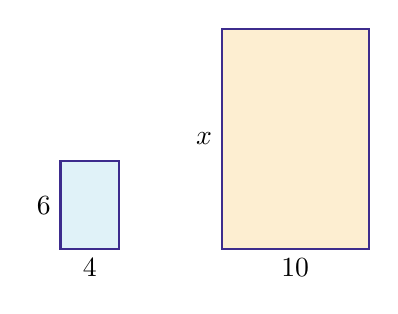
\begin{tikzpicture}[baseline=0pt]\filldraw[fill=fmkey!12,draw=fmtitle,thick] (0,0) rectangle (0.747,1.120);\node[below] at (0.373,0) {$4$};\node[left] at (0,0.560) {$6$};\filldraw[fill=fmturn!18,draw=fmtitle,thick] (2.047,0) rectangle (3.913,2.800);\node[below] at (2.980,0) {$10$};\node[left] at (2.047,1.400) {$x$};\end{tikzpicture}\par\vspace{3mm}\raggedright {\small\textbf{Method 1} --- Scale factor: \bk \quad $x = $ \bk}\par\vspace{2mm}{\small\textbf{Method 2} --- Proportion: $\dfrac{\bk}{\bk} = \dfrac{\bk}{\bk}$ \quad $x = $ \bk}\end{minipage}\hfill \begin{minipage}[t]{0.485\linewidth}\textbf{7.}\par\vspace{1mm}\centering 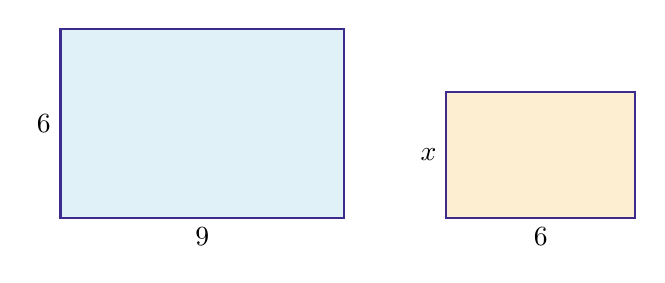
\begin{tikzpicture}[baseline=0pt]\filldraw[fill=fmkey!12,draw=fmtitle,thick] (0,0) rectangle (3.600,2.400);\node[below] at (1.800,0) {$9$};\node[left] at (0,1.200) {$6$};\filldraw[fill=fmturn!18,draw=fmtitle,thick] (4.900,0) rectangle (7.300,1.600);\node[below] at (6.100,0) {$6$};\node[left] at (4.900,0.800) {$x$};\end{tikzpicture}\par\vspace{3mm}\raggedright {\small\textbf{Method 1} --- Scale factor: \bk \quad $x = $ \bk}\par\vspace{2mm}{\small\textbf{Method 2} --- Proportion: $\dfrac{\bk}{\bk} = \dfrac{\bk}{\bk}$ \quad $x = $ \bk}\end{minipage}\par\vspace{14mm}
\needspace{6.2cm}\noindent \begin{minipage}[t]{0.485\linewidth}\textbf{8.}\par\vspace{1mm}\centering 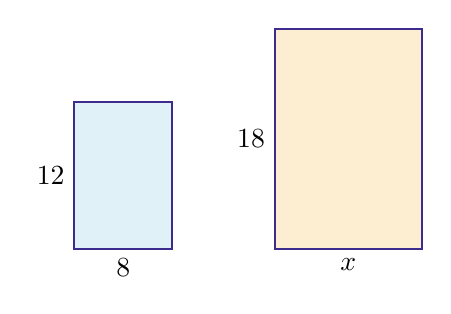
\begin{tikzpicture}[baseline=0pt]\filldraw[fill=fmkey!12,draw=fmtitle,thick] (0,0) rectangle (1.244,1.867);\node[below] at (0.622,0) {$8$};\node[left] at (0,0.933) {$12$};\filldraw[fill=fmturn!18,draw=fmtitle,thick] (2.544,0) rectangle (4.411,2.800);\node[below] at (3.478,0) {$x$};\node[left] at (2.544,1.400) {$18$};\end{tikzpicture}\par\vspace{3mm}\raggedright {\small\textbf{Method 1} --- Scale factor: \bk \quad $x = $ \bk}\par\vspace{2mm}{\small\textbf{Method 2} --- Proportion: $\dfrac{\bk}{\bk} = \dfrac{\bk}{\bk}$ \quad $x = $ \bk}\end{minipage}\hfill \begin{minipage}[t]{0.485\linewidth}\textbf{9.}\par\vspace{1mm}\centering 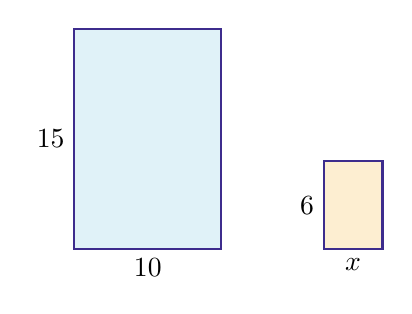
\begin{tikzpicture}[baseline=0pt]\filldraw[fill=fmkey!12,draw=fmtitle,thick] (0,0) rectangle (1.867,2.800);\node[below] at (0.933,0) {$10$};\node[left] at (0,1.400) {$15$};\filldraw[fill=fmturn!18,draw=fmtitle,thick] (3.167,0) rectangle (3.913,1.120);\node[below] at (3.540,0) {$x$};\node[left] at (3.167,0.560) {$6$};\end{tikzpicture}\par\vspace{3mm}\raggedright {\small\textbf{Method 1} --- Scale factor: \bk \quad $x = $ \bk}\par\vspace{2mm}{\small\textbf{Method 2} --- Proportion: $\dfrac{\bk}{\bk} = \dfrac{\bk}{\bk}$ \quad $x = $ \bk}\end{minipage}\par\vspace{14mm}
\needspace{6.2cm}\noindent \begin{minipage}[t]{0.485\linewidth}\textbf{10.}\par\vspace{1mm}\centering 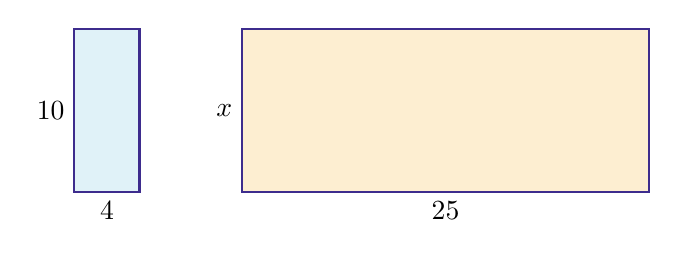
\begin{tikzpicture}[baseline=0pt]\filldraw[fill=fmkey!12,draw=fmtitle,thick] (0,0) rectangle (0.828,2.069);\node[below] at (0.414,0) {$4$};\node[left] at (0,1.034) {$10$};\filldraw[fill=fmturn!18,draw=fmtitle,thick] (2.128,0) rectangle (7.300,2.069);\node[below] at (4.714,0) {$25$};\node[left] at (2.128,1.034) {$x$};\end{tikzpicture}\par\vspace{3mm}\raggedright {\small\textbf{Method 1} --- Scale factor: \bk \quad $x = $ \bk}\par\vspace{2mm}{\small\textbf{Method 2} --- Proportion: $\dfrac{\bk}{\bk} = \dfrac{\bk}{\bk}$ \quad $x = $ \bk}\end{minipage}\par\vspace{14mm}
\newpage
\parttitle{B}{Similar Triangles}
\begin{keyidea}
Match the sides by size: \textbf{shortest $\leftrightarrow$ shortest, middle $\leftrightarrow$ middle, longest $\leftrightarrow$ longest}.
The triangles are similar when \textbf{all three} ratios are the same number (the scale factor).\par\vspace{1mm}
In a \textbf{similarity statement} $\triangle ABC \sim \triangle DEF$, the \textbf{order} of the letters shows which vertices match: $A \leftrightarrow D$, $B \leftrightarrow E$, $C \leftrightarrow F$.
\end{keyidea}
\begin{watchme}\textbf{Example 1 --- Are they similar?}\par\vspace{2mm}\begin{minipage}[c]{0.44\linewidth}\centering 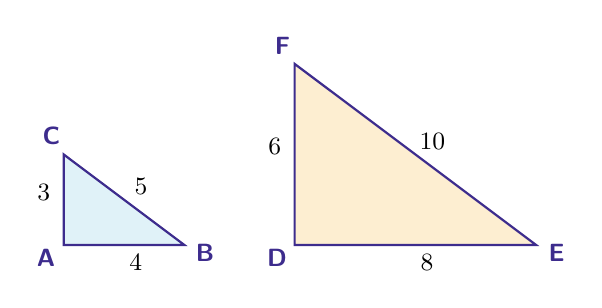
\begin{tikzpicture}[baseline=0pt]\filldraw[fill=fmkey!12,draw=fmtitle,thick] (0.000,0.000) -- (1.533,0.000) -- (0.000,1.150) -- cycle;\node[font=\small\bfseries,text=fmtitle] at (-0.224,-0.168) {A};\node[font=\small\bfseries,text=fmtitle] at (1.796,-0.098) {B};\node[font=\small\bfseries,text=fmtitle] at (-0.155,1.383) {C};\node[font=\small] at (0.916,-0.225) {$4$};\node[font=\small] at (0.983,0.737) {$5$};\node[font=\small] at (-0.253,0.670) {$3$};\filldraw[fill=fmturn!18,draw=fmtitle,thick] (2.933,0.000) -- (6.000,0.000) -- (2.933,2.300) -- cycle;\node[font=\small\bfseries,text=fmtitle] at (2.709,-0.168) {D};\node[font=\small\bfseries,text=fmtitle] at (6.262,-0.098) {E};\node[font=\small\bfseries,text=fmtitle] at (2.778,2.533) {F};\node[font=\small] at (4.616,-0.225) {$8$};\node[font=\small] at (4.683,1.312) {$10$};\node[font=\small] at (2.681,1.245) {$6$};\end{tikzpicture}\end{minipage}\hfill\begin{minipage}[c]{0.53\linewidth}Shortest: $\dfrac{6}{3}=2$ \quad Middle: $\dfrac{8}{4}=2$ \quad Longest: $\dfrac{10}{5}=2$\par\vspace{1mm}All three ratios are $2$, so the triangles \textbf{are similar}: \;$\mathbf{\triangle ABC \sim \triangle DEF}$, scale factor $\mathbf{2}$.\end{minipage}\end{watchme}
\begin{watchme}\textbf{Example 2 --- Find the missing side.} \;$\triangle ABC \sim \triangle DEF$.\par\vspace{2mm}\begin{minipage}[c]{0.44\linewidth}\centering 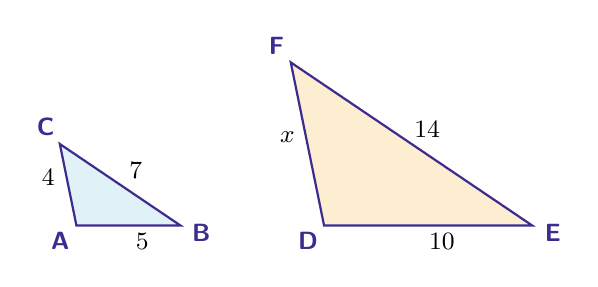
\begin{tikzpicture}[baseline=0pt]\filldraw[fill=fmkey!12,draw=fmtitle,thick] (0.211,0.000) -- (1.533,0.000) -- (0.000,1.036) -- cycle;\node[font=\small\bfseries,text=fmtitle] at (0.007,-0.191) {A};\node[font=\small\bfseries,text=fmtitle] at (1.797,-0.096) {B};\node[font=\small\bfseries,text=fmtitle] at (-0.180,1.250) {C};\node[font=\small] at (1.046,-0.207) {$5$};\node[font=\small] at (0.964,0.702) {$7$};\node[font=\small] at (-0.148,0.610) {$4$};\filldraw[fill=fmturn!18,draw=fmtitle,thick] (3.356,0.000) -- (6.000,0.000) -- (2.933,2.072) -- cycle;\node[font=\small\bfseries,text=fmtitle] at (3.152,-0.191) {D};\node[font=\small\bfseries,text=fmtitle] at (6.263,-0.096) {E};\node[font=\small\bfseries,text=fmtitle] at (2.753,2.286) {F};\node[font=\small] at (4.852,-0.207) {$10$};\node[font=\small] at (4.664,1.220) {$14$};\node[font=\small] at (2.891,1.128) {$x$};\end{tikzpicture}\end{minipage}\hfill\begin{minipage}[c]{0.53\linewidth}{\color{fmwatch}\textbf{Method 1 --- Scale factor}}\par\vspace{1.5mm} $AB \leftrightarrow DE$: \;$\dfrac{10}{5} = 2$.\par\vspace{1.5mm} $x = FD$ matches $CA = 4$: \;$x = 4 \times 2 = \mathbf{8}$.\par\vspace{2mm}{\color{fmwatch}\textbf{Method 2 --- Proportion}}\par\vspace{1.5mm} $\dfrac{DE}{AB} = \dfrac{FD}{CA}$\par\vspace{1.5mm} $\dfrac{10}{5} = \dfrac{x}{4}$ \;$\Rightarrow$\; $5x = 40$ \;$\Rightarrow$\; $x = \mathbf{8}$\end{minipage}\end{watchme}
\begin{mistake}
Checking only \textbf{two} pairs of sides is not enough. Sides $4, 6, 3$ and $8, 10, 6$ have two ratios equal to $2$,
but $\tfrac{10}{6} \neq 2$ --- so they are \textbf{not} similar. Check all three!
\end{mistake}
\newpage
\leveltag{fmwatch}{EASY}\quad{\color{fmtitle}\bfseries Triangles}\par\vspace{1mm}{\small Problems 1--5: Are the triangles similar? If yes, write a similarity statement. }\par\vspace{4mm}
\needspace{6.6cm}\noindent \begin{minipage}[t]{0.485\linewidth}\textbf{1.}\par\vspace{1mm}\centering 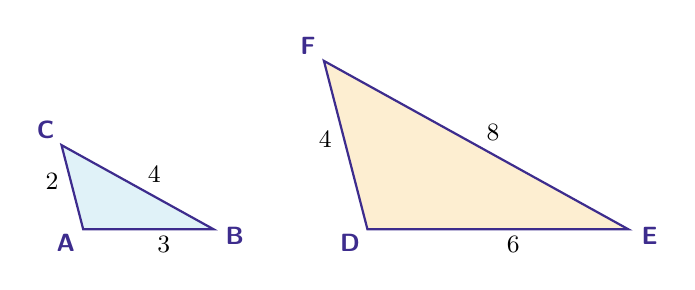
\begin{tikzpicture}[baseline=0pt]\filldraw[fill=fmkey!12,draw=fmtitle,thick] (0.276,0.000) -- (1.933,0.000) -- (0.000,1.070) -- cycle;\node[font=\small\bfseries,text=fmtitle] at (0.055,-0.171) {A};\node[font=\small\bfseries,text=fmtitle] at (2.202,-0.080) {B};\node[font=\small\bfseries,text=fmtitle] at (-0.201,1.264) {C};\node[font=\small] at (1.299,-0.188) {$3$};\node[font=\small] at (1.180,0.700) {$4$};\node[font=\small] at (-0.121,0.612) {$2$};\filldraw[fill=fmturn!18,draw=fmtitle,thick] (3.886,0.000) -- (7.200,0.000) -- (3.333,2.139) -- cycle;\node[font=\small\bfseries,text=fmtitle] at (3.664,-0.171) {D};\node[font=\small\bfseries,text=fmtitle] at (7.468,-0.080) {E};\node[font=\small\bfseries,text=fmtitle] at (3.132,2.334) {F};\node[font=\small] at (5.737,-0.188) {$6$};\node[font=\small] at (5.480,1.235) {$8$};\node[font=\small] at (3.351,1.147) {$4$};\end{tikzpicture}\par\vspace{3mm}\raggedright {\small Shortest: $\dfrac{\bk}{\bk}$ \; Middle: $\dfrac{\bk}{\bk}$ \; Longest: $\dfrac{\bk}{\bk}$}\par\vspace{1.5mm}{\small Similar? \; Yes \; / \; No \quad $\triangle$\lbk $\sim\triangle$\lbk}\end{minipage}\hfill \begin{minipage}[t]{0.485\linewidth}\textbf{2.}\par\vspace{1mm}\centering 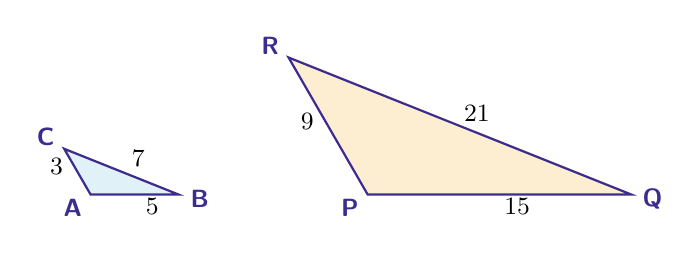
\begin{tikzpicture}[baseline=0pt]\filldraw[fill=fmkey!12,draw=fmtitle,thick] (0.335,0.000) -- (1.450,0.000) -- (0.000,0.580) -- cycle;\node[font=\small\bfseries,text=fmtitle] at (0.110,-0.167) {A};\node[font=\small\bfseries,text=fmtitle] at (1.723,-0.062) {B};\node[font=\small\bfseries,text=fmtitle] at (-0.235,0.732) {C};\node[font=\small] at (1.119,-0.147) {$5$};\node[font=\small] at (0.942,0.451) {$7$};\node[font=\small] at (-0.096,0.349) {$3$};\filldraw[fill=fmturn!18,draw=fmtitle,thick] (3.854,0.000) -- (7.200,0.000) -- (2.850,1.739) -- cycle;\node[font=\small\bfseries,text=fmtitle] at (3.629,-0.167) {P};\node[font=\small\bfseries,text=fmtitle] at (7.473,-0.062) {Q};\node[font=\small\bfseries,text=fmtitle] at (2.615,1.891) {R};\node[font=\small] at (5.753,-0.147) {$15$};\node[font=\small] at (5.242,1.030) {$21$};\node[font=\small] at (3.089,0.929) {$9$};\end{tikzpicture}\par\vspace{3mm}\raggedright {\small Shortest: $\dfrac{\bk}{\bk}$ \; Middle: $\dfrac{\bk}{\bk}$ \; Longest: $\dfrac{\bk}{\bk}$}\par\vspace{1.5mm}{\small Similar? \; Yes \; / \; No \quad $\triangle$\lbk $\sim\triangle$\lbk}\end{minipage}\par\vspace{12mm}
\needspace{6.6cm}\noindent \begin{minipage}[t]{0.485\linewidth}\textbf{3.}\par\vspace{1mm}\centering 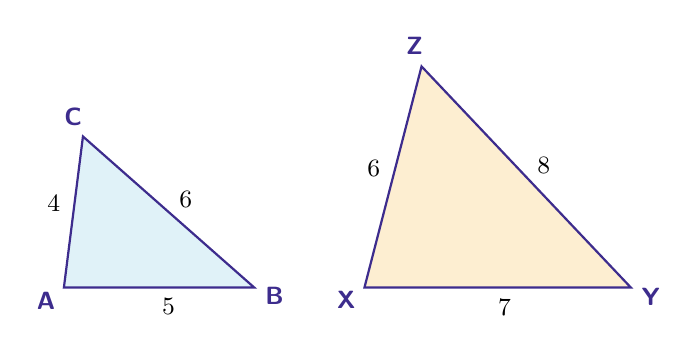
\begin{tikzpicture}[baseline=0pt]\filldraw[fill=fmkey!12,draw=fmtitle,thick] (0.000,0.000) -- (2.417,0.000) -- (0.242,1.918) -- cycle;\node[font=\small\bfseries,text=fmtitle] at (-0.227,-0.164) {A};\node[font=\small\bfseries,text=fmtitle] at (2.675,-0.108) {B};\node[font=\small\bfseries,text=fmtitle] at (0.116,2.168) {C};\node[font=\small] at (1.330,-0.241) {$5$};\node[font=\small] at (1.548,1.117) {$6$};\node[font=\small] at (-0.128,1.063) {$4$};\filldraw[fill=fmturn!18,draw=fmtitle,thick] (3.817,0.000) -- (7.200,0.000) -- (4.542,2.808) -- cycle;\node[font=\small\bfseries,text=fmtitle] at (3.586,-0.158) {X};\node[font=\small\bfseries,text=fmtitle] at (7.454,-0.118) {Y};\node[font=\small\bfseries,text=fmtitle] at (4.451,3.073) {Z};\node[font=\small] at (5.596,-0.255) {$7$};\node[font=\small] at (6.094,1.556) {$8$};\node[font=\small] at (3.934,1.518) {$6$};\end{tikzpicture}\par\vspace{3mm}\raggedright {\small Shortest: $\dfrac{\bk}{\bk}$ \; Middle: $\dfrac{\bk}{\bk}$ \; Longest: $\dfrac{\bk}{\bk}$}\par\vspace{1.5mm}{\small Similar? \; Yes \; / \; No \quad $\triangle$\lbk $\sim\triangle$\lbk}\end{minipage}\hfill \begin{minipage}[t]{0.485\linewidth}\textbf{4.}\par\vspace{1mm}\centering 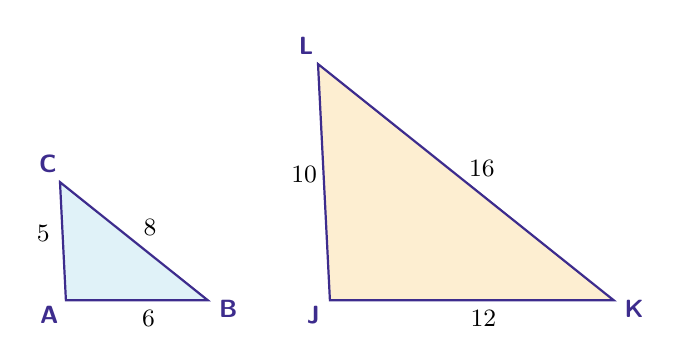
\begin{tikzpicture}[baseline=0pt]\filldraw[fill=fmkey!12,draw=fmtitle,thick] (0.075,0.000) -- (1.877,0.000) -- (0.000,1.500) -- cycle;\node[font=\small\bfseries,text=fmtitle] at (-0.136,-0.184) {A};\node[font=\small\bfseries,text=fmtitle] at (2.137,-0.106) {B};\node[font=\small\bfseries,text=fmtitle] at (-0.153,1.735) {C};\node[font=\small] at (1.123,-0.226) {$6$};\node[font=\small] at (1.143,0.927) {$8$};\node[font=\small] at (-0.212,0.852) {$5$};\filldraw[fill=fmturn!18,draw=fmtitle,thick] (3.428,0.000) -- (7.032,0.000) -- (3.277,3.000) -- cycle;\node[font=\small\bfseries,text=fmtitle] at (3.216,-0.184) {J};\node[font=\small\bfseries,text=fmtitle] at (7.291,-0.106) {K};\node[font=\small\bfseries,text=fmtitle] at (3.125,3.235) {L};\node[font=\small] at (5.377,-0.226) {$12$};\node[font=\small] at (5.359,1.677) {$16$};\node[font=\small] at (3.102,1.602) {$10$};\end{tikzpicture}\par\vspace{3mm}\raggedright {\small Shortest: $\dfrac{\bk}{\bk}$ \; Middle: $\dfrac{\bk}{\bk}$ \; Longest: $\dfrac{\bk}{\bk}$}\par\vspace{1.5mm}{\small Similar? \; Yes \; / \; No \quad $\triangle$\lbk $\sim\triangle$\lbk}\end{minipage}\par\vspace{12mm}
\needspace{6.6cm}\noindent \begin{minipage}[t]{0.485\linewidth}\textbf{5.}\par\vspace{1mm}\centering 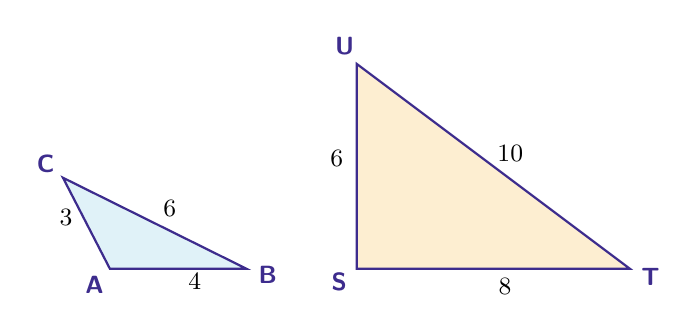
\begin{tikzpicture}[baseline=0pt]\filldraw[fill=fmkey!12,draw=fmtitle,thick] (0.596,0.000) -- (2.331,0.000) -- (0.000,1.156) -- cycle;\node[font=\small\bfseries,text=fmtitle] at (0.400,-0.200) {A};\node[font=\small\bfseries,text=fmtitle] at (2.600,-0.077) {B};\node[font=\small\bfseries,text=fmtitle] at (-0.220,1.330) {C};\node[font=\small] at (1.675,-0.167) {$4$};\node[font=\small] at (1.355,0.771) {$6$};\node[font=\small] at (0.038,0.652) {$3$};\filldraw[fill=fmturn!18,draw=fmtitle,thick] (3.731,0.000) -- (7.200,0.000) -- (3.731,2.602) -- cycle;\node[font=\small\bfseries,text=fmtitle] at (3.507,-0.168) {S};\node[font=\small\bfseries,text=fmtitle] at (7.462,-0.098) {T};\node[font=\small\bfseries,text=fmtitle] at (3.576,2.835) {U};\node[font=\small] at (5.615,-0.225) {$8$};\node[font=\small] at (5.681,1.463) {$10$};\node[font=\small] at (3.478,1.396) {$6$};\end{tikzpicture}\par\vspace{3mm}\raggedright {\small Shortest: $\dfrac{\bk}{\bk}$ \; Middle: $\dfrac{\bk}{\bk}$ \; Longest: $\dfrac{\bk}{\bk}$}\par\vspace{1.5mm}{\small Similar? \; Yes \; / \; No \quad $\triangle$\lbk $\sim\triangle$\lbk}\end{minipage}\par\vspace{12mm}
\newpage
\leveltag{fmwatch}{EASY}\quad{\color{fmtitle}\bfseries Triangles --- Find the Missing Side}\par\vspace{1mm}{\small The triangles are similar. Find $x$ two ways: with the scale factor and with a proportion.}\par\vspace{5mm}
\needspace{6.5cm}\noindent \begin{minipage}[t]{0.485\linewidth}\textbf{6.}\par\vspace{1mm}\centering 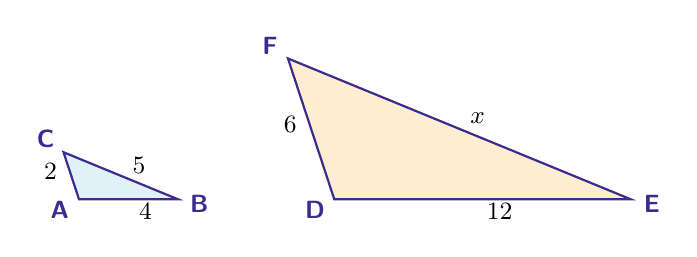
\begin{tikzpicture}[baseline=0pt]\filldraw[fill=fmkey!12,draw=fmtitle,thick] (0.196,0.000) -- (1.450,0.000) -- (0.000,0.596) -- cycle;\node[font=\small\bfseries,text=fmtitle] at (-0.048,-0.137) {A};\node[font=\small\bfseries,text=fmtitle] at (1.723,-0.060) {B};\node[font=\small\bfseries,text=fmtitle] at (-0.227,0.760) {C};\node[font=\small] at (1.042,-0.158) {$4$};\node[font=\small] at (0.960,0.430) {$5$};\node[font=\small] at (-0.166,0.356) {$2$};\filldraw[fill=fmturn!18,draw=fmtitle,thick] (3.438,0.000) -- (7.200,0.000) -- (2.850,1.787) -- cycle;\node[font=\small\bfseries,text=fmtitle] at (3.194,-0.137) {D};\node[font=\small\bfseries,text=fmtitle] at (7.473,-0.060) {E};\node[font=\small\bfseries,text=fmtitle] at (2.623,1.951) {F};\node[font=\small] at (5.538,-0.158) {$12$};\node[font=\small] at (5.260,1.026) {$x$};\node[font=\small] at (2.880,0.952) {$6$};\end{tikzpicture}\par\vspace{3mm}\raggedright {\small $\triangle ABC \sim \triangle DEF$}\par\vspace{1mm}{\small\textbf{Method 1} --- Scale factor: \bk \quad $x = $ \bk}\par\vspace{2mm}{\small\textbf{Method 2} --- Proportion: $\dfrac{\bk}{\bk} = \dfrac{\bk}{\bk}$ \quad $x = $ \bk}\end{minipage}\hfill \begin{minipage}[t]{0.485\linewidth}\textbf{7.}\par\vspace{1mm}\centering 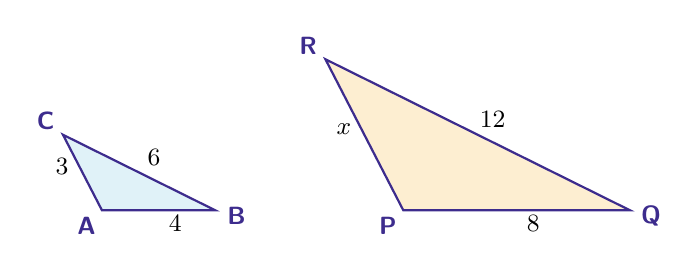
\begin{tikzpicture}[baseline=0pt]\filldraw[fill=fmkey!12,draw=fmtitle,thick] (0.495,0.000) -- (1.933,0.000) -- (0.000,0.959) -- cycle;\node[font=\small\bfseries,text=fmtitle] at (0.298,-0.200) {A};\node[font=\small\bfseries,text=fmtitle] at (2.203,-0.077) {B};\node[font=\small\bfseries,text=fmtitle] at (-0.220,1.133) {C};\node[font=\small] at (1.426,-0.167) {$4$};\node[font=\small] at (1.156,0.672) {$6$};\node[font=\small] at (-0.012,0.553) {$3$};\filldraw[fill=fmturn!18,draw=fmtitle,thick] (4.322,0.000) -- (7.200,0.000) -- (3.333,1.918) -- cycle;\node[font=\small\bfseries,text=fmtitle] at (4.126,-0.200) {P};\node[font=\small\bfseries,text=fmtitle] at (7.469,-0.077) {Q};\node[font=\small\bfseries,text=fmtitle] at (3.114,2.092) {R};\node[font=\small] at (5.973,-0.167) {$8$};\node[font=\small] at (5.456,1.151) {$12$};\node[font=\small] at (3.568,1.033) {$x$};\end{tikzpicture}\par\vspace{3mm}\raggedright {\small $\triangle ABC \sim \triangle PQR$}\par\vspace{1mm}{\small\textbf{Method 1} --- Scale factor: \bk \quad $x = $ \bk}\par\vspace{2mm}{\small\textbf{Method 2} --- Proportion: $\dfrac{\bk}{\bk} = \dfrac{\bk}{\bk}$ \quad $x = $ \bk}\end{minipage}\par\vspace{4mm}
\needspace{6.5cm}\noindent \begin{minipage}[t]{0.485\linewidth}\textbf{8.}\par\vspace{1mm}\centering 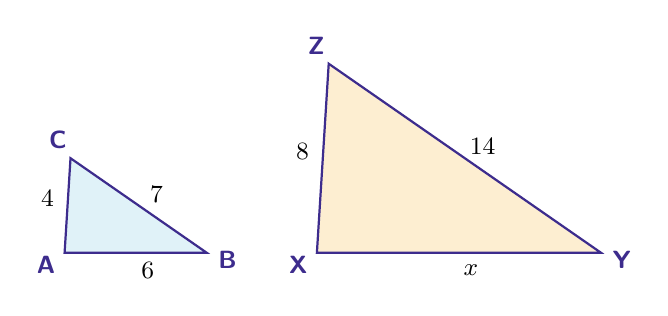
\begin{tikzpicture}[baseline=0pt]\filldraw[fill=fmkey!12,draw=fmtitle,thick] (0.000,0.000) -- (1.804,0.000) -- (0.075,1.200) -- cycle;\node[font=\small\bfseries,text=fmtitle] at (-0.236,-0.151) {A};\node[font=\small\bfseries,text=fmtitle] at (2.069,-0.090) {B};\node[font=\small\bfseries,text=fmtitle] at (-0.084,1.431) {C};\node[font=\small] at (1.055,-0.222) {$6$};\node[font=\small] at (1.167,0.745) {$7$};\node[font=\small] at (-0.218,0.687) {$4$};\filldraw[fill=fmturn!18,draw=fmtitle,thick] (3.204,0.000) -- (6.811,0.000) -- (3.354,2.400) -- cycle;\node[font=\small\bfseries,text=fmtitle] at (2.968,-0.151) {X};\node[font=\small\bfseries,text=fmtitle] at (7.076,-0.090) {Y};\node[font=\small\bfseries,text=fmtitle] at (3.195,2.631) {Z};\node[font=\small] at (5.160,-0.222) {$x$};\node[font=\small] at (5.310,1.345) {$14$};\node[font=\small] at (3.023,1.287) {$8$};\end{tikzpicture}\par\vspace{3mm}\raggedright {\small $\triangle ABC \sim \triangle XYZ$}\par\vspace{1mm}{\small\textbf{Method 1} --- Scale factor: \bk \quad $x = $ \bk}\par\vspace{2mm}{\small\textbf{Method 2} --- Proportion: $\dfrac{\bk}{\bk} = \dfrac{\bk}{\bk}$ \quad $x = $ \bk}\end{minipage}\hfill \begin{minipage}[t]{0.485\linewidth}\textbf{9.}\par\vspace{1mm}\centering 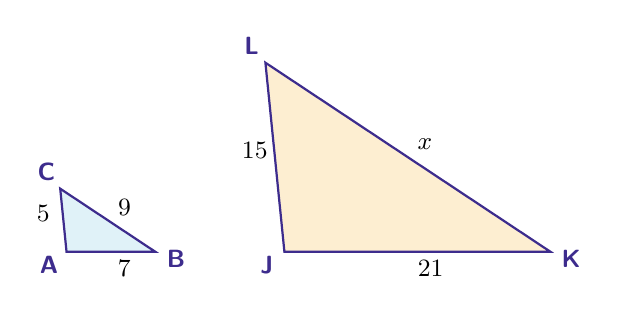
\begin{tikzpicture}[baseline=0pt]\filldraw[fill=fmkey!12,draw=fmtitle,thick] (0.080,0.000) -- (1.206,0.000) -- (0.000,0.800) -- cycle;\node[font=\small\bfseries,text=fmtitle] at (-0.142,-0.170) {A};\node[font=\small\bfseries,text=fmtitle] at (1.471,-0.091) {B};\node[font=\small\bfseries,text=fmtitle] at (-0.175,1.018) {C};\node[font=\small] at (0.812,-0.210) {$7$};\node[font=\small] at (0.817,0.564) {$9$};\node[font=\small] at (-0.215,0.488) {$5$};\filldraw[fill=fmturn!18,draw=fmtitle,thick] (2.847,0.000) -- (6.224,0.000) -- (2.606,2.400) -- cycle;\node[font=\small\bfseries,text=fmtitle] at (2.625,-0.170) {J};\node[font=\small\bfseries,text=fmtitle] at (6.489,-0.091) {K};\node[font=\small\bfseries,text=fmtitle] at (2.431,2.618) {L};\node[font=\small] at (4.705,-0.210) {$21$};\node[font=\small] at (4.630,1.364) {$x$};\node[font=\small] at (2.471,1.288) {$15$};\end{tikzpicture}\par\vspace{3mm}\raggedright {\small $\triangle ABC \sim \triangle JKL$}\par\vspace{1mm}{\small\textbf{Method 1} --- Scale factor: \bk \quad $x = $ \bk}\par\vspace{2mm}{\small\textbf{Method 2} --- Proportion: $\dfrac{\bk}{\bk} = \dfrac{\bk}{\bk}$ \quad $x = $ \bk}\end{minipage}\par\vspace{4mm}
\needspace{6.5cm}\noindent \begin{minipage}[t]{0.485\linewidth}\textbf{10.}\par\vspace{1mm}\centering 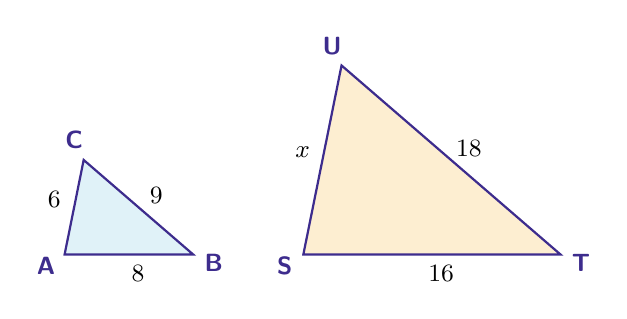
\begin{tikzpicture}[baseline=0pt]\filldraw[fill=fmkey!12,draw=fmtitle,thick] (0.000,0.000) -- (1.632,0.000) -- (0.242,1.200) -- cycle;\node[font=\small\bfseries,text=fmtitle] at (-0.236,-0.151) {A};\node[font=\small\bfseries,text=fmtitle] at (1.893,-0.103) {B};\node[font=\small\bfseries,text=fmtitle] at (0.121,1.453) {C};\node[font=\small] at (0.933,-0.244) {$8$};\node[font=\small] at (1.165,0.746) {$9$};\node[font=\small] at (-0.130,0.700) {$6$};\filldraw[fill=fmturn!18,draw=fmtitle,thick] (3.032,0.000) -- (6.297,0.000) -- (3.517,2.400) -- cycle;\node[font=\small\bfseries,text=fmtitle] at (2.796,-0.151) {S};\node[font=\small\bfseries,text=fmtitle] at (6.557,-0.103) {T};\node[font=\small\bfseries,text=fmtitle] at (3.396,2.653) {U};\node[font=\small] at (4.781,-0.244) {$16$};\node[font=\small] at (5.134,1.346) {$18$};\node[font=\small] at (3.024,1.300) {$x$};\end{tikzpicture}\par\vspace{3mm}\raggedright {\small $\triangle ABC \sim \triangle STU$}\par\vspace{1mm}{\small\textbf{Method 1} --- Scale factor: \bk \quad $x = $ \bk}\par\vspace{2mm}{\small\textbf{Method 2} --- Proportion: $\dfrac{\bk}{\bk} = \dfrac{\bk}{\bk}$ \quad $x = $ \bk}\end{minipage}\par\vspace{4mm}
\newpage
\leveltag{fmturn}{MEDIUM}\quad{\color{fmtitle}\bfseries Triangles}\par\vspace{1mm}{\small Problems 1--5: Are the triangles similar? A triangle may be turned or flipped, so match sides by \textbf{size}, not by position.}\par\vspace{4mm}
\needspace{6.6cm}\noindent \begin{minipage}[t]{0.485\linewidth}\textbf{1.}\par\vspace{1mm}\centering 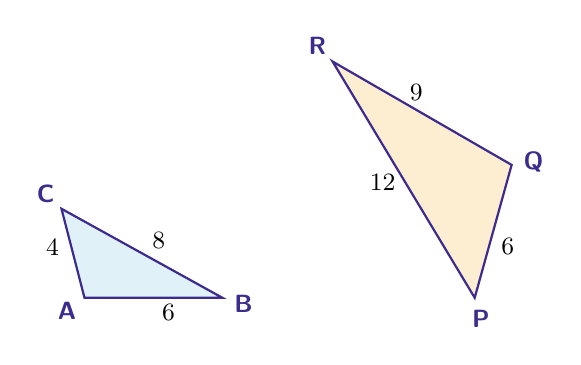
\begin{tikzpicture}[baseline=0pt]\filldraw[fill=fmkey!12,draw=fmtitle,thick] (0.292,0.000) -- (2.043,0.000) -- (0.000,1.130) -- cycle;\node[font=\small\bfseries,text=fmtitle] at (0.070,-0.171) {A};\node[font=\small\bfseries,text=fmtitle] at (2.311,-0.080) {B};\node[font=\small\bfseries,text=fmtitle] at (-0.201,1.325) {C};\node[font=\small] at (1.361,-0.188) {$6$};\node[font=\small] at (1.235,0.730) {$8$};\node[font=\small] at (-0.113,0.642) {$4$};\filldraw[fill=fmturn!18,draw=fmtitle,thick] (5.717,1.687) -- (3.443,3.000) -- (5.248,0.000) -- cycle;\node[font=\small\bfseries,text=fmtitle] at (5.994,1.725) {Q};\node[font=\small\bfseries,text=fmtitle] at (3.250,3.203) {R};\node[font=\small\bfseries,text=fmtitle] at (5.325,-0.269) {P};\node[font=\small] at (4.506,2.603) {$9$};\node[font=\small] at (4.078,1.464) {$12$};\node[font=\small] at (5.668,0.647) {$6$};\end{tikzpicture}\par\vspace{3mm}\raggedright {\small Shortest: $\dfrac{\bk}{\bk}$ \; Middle: $\dfrac{\bk}{\bk}$ \; Longest: $\dfrac{\bk}{\bk}$}\par\vspace{1.5mm}{\small Similar? \; Yes \; / \; No \quad $\triangle$\lbk $\sim\triangle$\lbk}\end{minipage}\hfill \begin{minipage}[t]{0.485\linewidth}\textbf{2.}\par\vspace{1mm}\centering 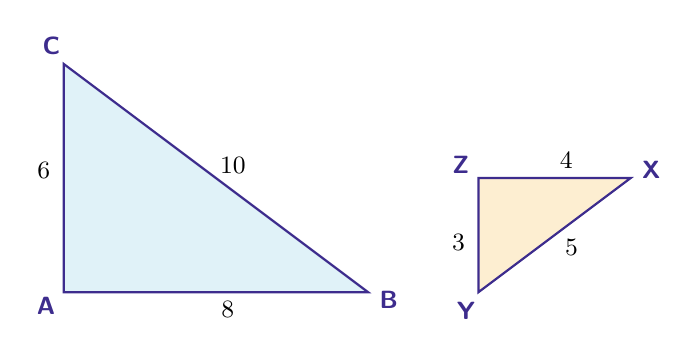
\begin{tikzpicture}[baseline=0pt]\filldraw[fill=fmkey!12,draw=fmtitle,thick] (0.000,0.000) -- (3.867,0.000) -- (0.000,2.900) -- cycle;\node[font=\small\bfseries,text=fmtitle] at (-0.224,-0.168) {A};\node[font=\small\bfseries,text=fmtitle] at (4.129,-0.098) {B};\node[font=\small\bfseries,text=fmtitle] at (-0.155,3.133) {C};\node[font=\small] at (2.083,-0.225) {$8$};\node[font=\small] at (2.149,1.612) {$10$};\node[font=\small] at (-0.253,1.545) {$6$};\filldraw[fill=fmturn!18,draw=fmtitle,thick] (5.267,1.450) -- (7.200,1.450) -- (5.267,0.000) -- cycle;\node[font=\small\bfseries,text=fmtitle] at (5.043,1.618) {Z};\node[font=\small\bfseries,text=fmtitle] at (7.462,1.548) {X};\node[font=\small\bfseries,text=fmtitle] at (5.111,-0.233) {Y};\node[font=\small] at (6.383,1.675) {$4$};\node[font=\small] at (6.449,0.563) {$5$};\node[font=\small] at (5.014,0.630) {$3$};\end{tikzpicture}\par\vspace{3mm}\raggedright {\small Shortest: $\dfrac{\bk}{\bk}$ \; Middle: $\dfrac{\bk}{\bk}$ \; Longest: $\dfrac{\bk}{\bk}$}\par\vspace{1.5mm}{\small Similar? \; Yes \; / \; No \quad $\triangle$\lbk $\sim\triangle$\lbk}\end{minipage}\par\vspace{12mm}
\needspace{6.6cm}\noindent \begin{minipage}[t]{0.485\linewidth}\textbf{3.}\par\vspace{1mm}\centering 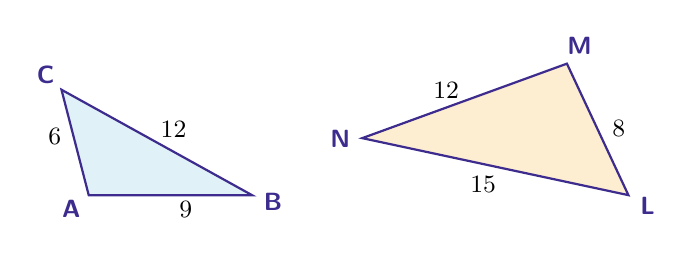
\begin{tikzpicture}[baseline=0pt]\filldraw[fill=fmkey!12,draw=fmtitle,thick] (0.346,0.000) -- (2.420,0.000) -- (0.000,1.339) -- cycle;\node[font=\small\bfseries,text=fmtitle] at (0.124,-0.171) {A};\node[font=\small\bfseries,text=fmtitle] at (2.688,-0.080) {B};\node[font=\small\bfseries,text=fmtitle] at (-0.201,1.534) {C};\node[font=\small] at (1.577,-0.188) {$9$};\node[font=\small] at (1.423,0.835) {$12$};\node[font=\small] at (-0.086,0.747) {$6$};\filldraw[fill=fmturn!18,draw=fmtitle,thick] (6.419,1.670) -- (3.820,0.724) -- (7.200,0.000) -- cycle;\node[font=\small\bfseries,text=fmtitle] at (6.578,1.900) {M};\node[font=\small\bfseries,text=fmtitle] at (3.540,0.714) {N};\node[font=\small\bfseries,text=fmtitle] at (7.443,-0.140) {L};\node[font=\small] at (4.885,1.332) {$12$};\node[font=\small] at (5.356,0.140) {$15$};\node[font=\small] at (7.079,0.845) {$8$};\end{tikzpicture}\par\vspace{3mm}\raggedright {\small Shortest: $\dfrac{\bk}{\bk}$ \; Middle: $\dfrac{\bk}{\bk}$ \; Longest: $\dfrac{\bk}{\bk}$}\par\vspace{1.5mm}{\small Similar? \; Yes \; / \; No \quad $\triangle$\lbk $\sim\triangle$\lbk}\end{minipage}\hfill \begin{minipage}[t]{0.485\linewidth}\textbf{4.}\par\vspace{1mm}\centering 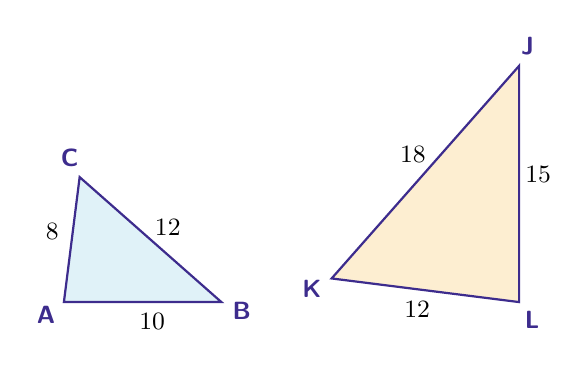
\begin{tikzpicture}[baseline=0pt]\filldraw[fill=fmkey!12,draw=fmtitle,thick] (0.000,0.000) -- (2.000,0.000) -- (0.200,1.587) -- cycle;\node[font=\small\bfseries,text=fmtitle] at (-0.227,-0.164) {A};\node[font=\small\bfseries,text=fmtitle] at (2.258,-0.108) {B};\node[font=\small\bfseries,text=fmtitle] at (0.074,1.837) {C};\node[font=\small] at (1.122,-0.241) {$10$};\node[font=\small] at (1.319,0.952) {$12$};\node[font=\small] at (-0.149,0.898) {$8$};\filldraw[fill=fmturn!18,draw=fmtitle,thick] (5.781,0.000) -- (5.781,3.000) -- (3.400,0.300) -- cycle;\node[font=\small\bfseries,text=fmtitle] at (5.945,-0.227) {L};\node[font=\small\bfseries,text=fmtitle] at (5.889,3.258) {J};\node[font=\small\bfseries,text=fmtitle] at (3.150,0.174) {K};\node[font=\small] at (6.022,1.622) {$15$};\node[font=\small] at (4.433,1.869) {$18$};\node[font=\small] at (4.487,-0.099) {$12$};\end{tikzpicture}\par\vspace{3mm}\raggedright {\small Shortest: $\dfrac{\bk}{\bk}$ \; Middle: $\dfrac{\bk}{\bk}$ \; Longest: $\dfrac{\bk}{\bk}$}\par\vspace{1.5mm}{\small Similar? \; Yes \; / \; No \quad $\triangle$\lbk $\sim\triangle$\lbk}\end{minipage}\par\vspace{12mm}
\needspace{6.6cm}\noindent \begin{minipage}[t]{0.485\linewidth}\textbf{5.}\par\vspace{1mm}\centering 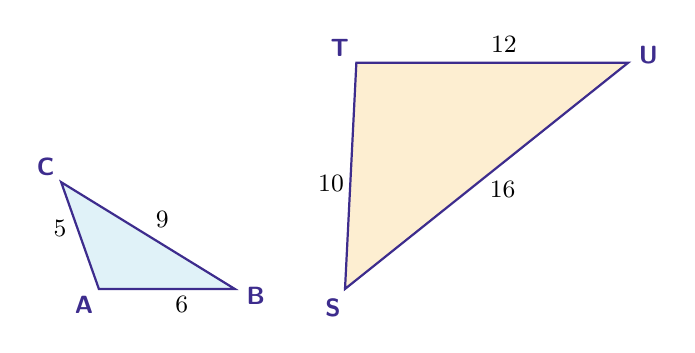
\begin{tikzpicture}[baseline=0pt]\filldraw[fill=fmkey!12,draw=fmtitle,thick] (0.479,0.000) -- (2.205,0.000) -- (0.000,1.356) -- cycle;\node[font=\small\bfseries,text=fmtitle] at (0.290,-0.206) {A};\node[font=\small\bfseries,text=fmtitle] at (2.470,-0.091) {B};\node[font=\small\bfseries,text=fmtitle] at (-0.197,1.555) {C};\node[font=\small] at (1.532,-0.192) {$6$};\node[font=\small] at (1.285,0.877) {$9$};\node[font=\small] at (-0.016,0.766) {$5$};\filldraw[fill=fmturn!18,draw=fmtitle,thick] (3.749,2.872) -- (7.200,2.872) -- (3.605,0.000) -- cycle;\node[font=\small\bfseries,text=fmtitle] at (3.537,3.056) {T};\node[font=\small\bfseries,text=fmtitle] at (7.459,2.978) {U};\node[font=\small\bfseries,text=fmtitle] at (3.452,-0.235) {S};\node[font=\small] at (5.622,3.099) {$12$};\node[font=\small] at (5.606,1.259) {$16$};\node[font=\small] at (3.427,1.334) {$10$};\end{tikzpicture}\par\vspace{3mm}\raggedright {\small Shortest: $\dfrac{\bk}{\bk}$ \; Middle: $\dfrac{\bk}{\bk}$ \; Longest: $\dfrac{\bk}{\bk}$}\par\vspace{1.5mm}{\small Similar? \; Yes \; / \; No \quad $\triangle$\lbk $\sim\triangle$\lbk}\end{minipage}\par\vspace{12mm}
\newpage
\leveltag{fmturn}{MEDIUM}\quad{\color{fmtitle}\bfseries Triangles --- Find the Missing Side}\par\vspace{1mm}{\small Use the similarity statement to match sides (the triangles may be turned or flipped), then find $x$ two ways.}\par\vspace{5mm}
\needspace{6.5cm}\noindent \begin{minipage}[t]{0.485\linewidth}\textbf{6.}\par\vspace{1mm}\centering 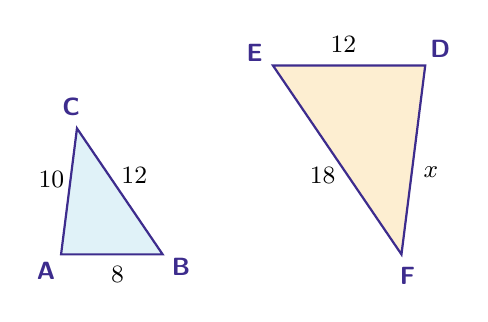
\begin{tikzpicture}[baseline=0pt]\filldraw[fill=fmkey!12,draw=fmtitle,thick] (0.000,0.000) -- (1.290,0.000) -- (0.202,1.600) -- cycle;\node[font=\small\bfseries,text=fmtitle] at (-0.191,-0.205) {A};\node[font=\small\bfseries,text=fmtitle] at (1.522,-0.156) {B};\node[font=\small\bfseries,text=fmtitle] at (0.127,1.870) {C};\node[font=\small] at (0.717,-0.260) {$8$};\node[font=\small] at (0.930,0.997) {$12$};\node[font=\small] at (-0.123,0.951) {$10$};\filldraw[fill=fmturn!18,draw=fmtitle,thick] (4.625,2.400) -- (2.690,2.400) -- (4.323,0.000) -- cycle;\node[font=\small\bfseries,text=fmtitle] at (4.816,2.605) {D};\node[font=\small\bfseries,text=fmtitle] at (2.458,2.556) {E};\node[font=\small\bfseries,text=fmtitle] at (4.398,-0.270) {F};\node[font=\small] at (3.586,2.660) {$12$};\node[font=\small] at (3.322,1.003) {$18$};\node[font=\small] at (4.698,1.049) {$x$};\end{tikzpicture}\par\vspace{3mm}\raggedright {\small $\triangle ABC \sim \triangle DEF$}\par\vspace{1mm}{\small\textbf{Method 1} --- Scale factor: \bk \quad $x = $ \bk}\par\vspace{2mm}{\small\textbf{Method 2} --- Proportion: $\dfrac{\bk}{\bk} = \dfrac{\bk}{\bk}$ \quad $x = $ \bk}\end{minipage}\hfill \begin{minipage}[t]{0.485\linewidth}\textbf{7.}\par\vspace{1mm}\centering 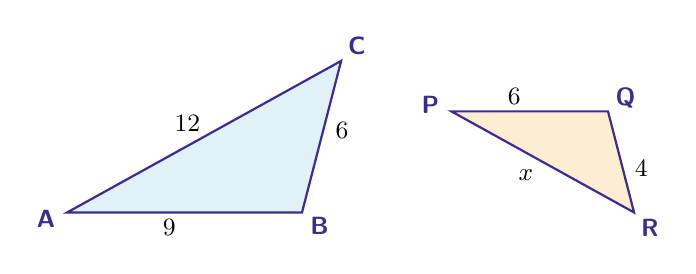
\begin{tikzpicture}[baseline=0pt]\filldraw[fill=fmkey!12,draw=fmtitle,thick] (0.000,0.000) -- (2.983,0.000) -- (3.480,1.925) -- cycle;\node[font=\small\bfseries,text=fmtitle] at (-0.268,-0.080) {A};\node[font=\small\bfseries,text=fmtitle] at (3.204,-0.171) {B};\node[font=\small\bfseries,text=fmtitle] at (3.681,2.120) {C};\node[font=\small] at (1.297,-0.188) {$9$};\node[font=\small] at (3.490,1.040) {$6$};\node[font=\small] at (1.527,1.128) {$12$};\filldraw[fill=fmturn!18,draw=fmtitle,thick] (4.880,1.284) -- (6.869,1.284) -- (7.200,0.000) -- cycle;\node[font=\small\bfseries,text=fmtitle] at (4.612,1.364) {P};\node[font=\small\bfseries,text=fmtitle] at (7.090,1.455) {Q};\node[font=\small\bfseries,text=fmtitle] at (7.401,-0.195) {R};\node[font=\small] at (5.680,1.471) {$6$};\node[font=\small] at (7.293,0.565) {$4$};\node[font=\small] at (5.827,0.476) {$x$};\end{tikzpicture}\par\vspace{3mm}\raggedright {\small $\triangle ABC \sim \triangle PQR$}\par\vspace{1mm}{\small\textbf{Method 1} --- Scale factor: \bk \quad $x = $ \bk}\par\vspace{2mm}{\small\textbf{Method 2} --- Proportion: $\dfrac{\bk}{\bk} = \dfrac{\bk}{\bk}$ \quad $x = $ \bk}\end{minipage}\par\vspace{4mm}
\needspace{6.5cm}\noindent \begin{minipage}[t]{0.485\linewidth}\textbf{8.}\par\vspace{1mm}\centering 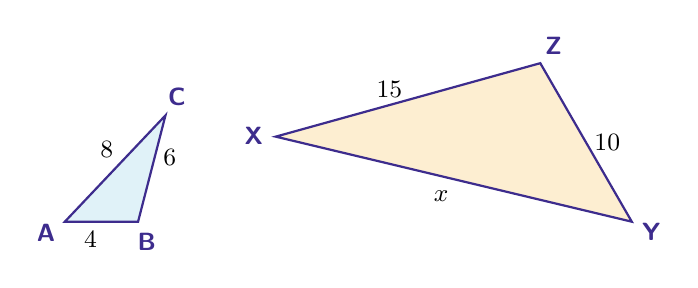
\begin{tikzpicture}[baseline=0pt]\filldraw[fill=fmkey!12,draw=fmtitle,thick] (0.000,0.000) -- (0.930,0.000) -- (1.278,1.350) -- cycle;\node[font=\small\bfseries,text=fmtitle] at (-0.239,-0.146) {A};\node[font=\small\bfseries,text=fmtitle] at (1.040,-0.257) {B};\node[font=\small\bfseries,text=fmtitle] at (1.423,1.590) {C};\node[font=\small] at (0.326,-0.231) {$4$};\node[font=\small] at (1.334,0.816) {$6$};\node[font=\small] at (0.532,0.923) {$8$};\filldraw[fill=fmturn!18,draw=fmtitle,thick] (7.200,0.000) -- (6.038,2.013) -- (2.678,1.080) -- cycle;\node[font=\small\bfseries,text=fmtitle] at (7.446,-0.134) {Y};\node[font=\small\bfseries,text=fmtitle] at (6.205,2.237) {Z};\node[font=\small\bfseries,text=fmtitle] at (2.398,1.085) {X};\node[font=\small] at (6.889,1.001) {$10$};\node[font=\small] at (4.121,1.675) {$15$};\node[font=\small] at (4.778,0.324) {$x$};\end{tikzpicture}\par\vspace{3mm}\raggedright {\small $\triangle ABC \sim \triangle YZX$}\par\vspace{1mm}{\small\textbf{Method 1} --- Scale factor: \bk \quad $x = $ \bk}\par\vspace{2mm}{\small\textbf{Method 2} --- Proportion: $\dfrac{\bk}{\bk} = \dfrac{\bk}{\bk}$ \quad $x = $ \bk}\end{minipage}\hfill \begin{minipage}[t]{0.485\linewidth}\textbf{9.}\par\vspace{1mm}\centering 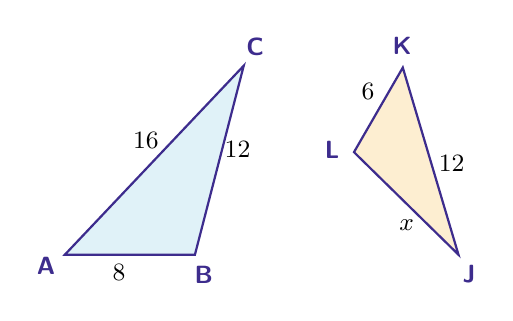
\begin{tikzpicture}[baseline=0pt]\filldraw[fill=fmkey!12,draw=fmtitle,thick] (0.000,0.000) -- (1.652,0.000) -- (2.272,2.400) -- cycle;\node[font=\small\bfseries,text=fmtitle] at (-0.239,-0.146) {A};\node[font=\small\bfseries,text=fmtitle] at (1.763,-0.257) {B};\node[font=\small\bfseries,text=fmtitle] at (2.417,2.640) {C};\node[font=\small] at (0.687,-0.231) {$8$};\node[font=\small] at (2.193,1.341) {$12$};\node[font=\small] at (1.029,1.448) {$16$};\filldraw[fill=fmturn!18,draw=fmtitle,thick] (4.292,2.376) -- (3.672,1.302) -- (4.999,0.000) -- cycle;\node[font=\small\bfseries,text=fmtitle] at (4.285,2.656) {K};\node[font=\small\bfseries,text=fmtitle] at (3.394,1.335) {L};\node[font=\small\bfseries,text=fmtitle] at (5.134,-0.245) {J};\node[font=\small] at (3.851,2.075) {$6$};\node[font=\small] at (4.342,0.381) {$x$};\node[font=\small] at (4.913,1.156) {$12$};\end{tikzpicture}\par\vspace{3mm}\raggedright {\small $\triangle ABC \sim \triangle KLJ$}\par\vspace{1mm}{\small\textbf{Method 1} --- Scale factor: \bk \quad $x = $ \bk}\par\vspace{2mm}{\small\textbf{Method 2} --- Proportion: $\dfrac{\bk}{\bk} = \dfrac{\bk}{\bk}$ \quad $x = $ \bk}\end{minipage}\par\vspace{4mm}
\needspace{6.5cm}\noindent \begin{minipage}[t]{0.485\linewidth}\textbf{10.}\par\vspace{1mm}\centering 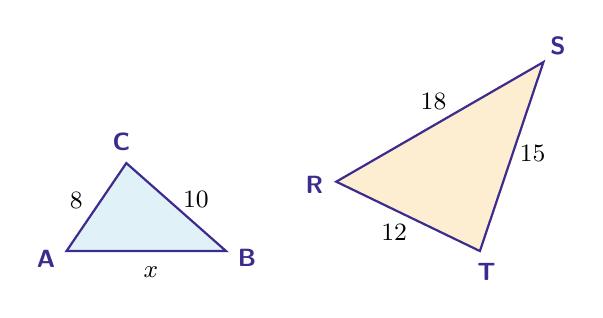
\begin{tikzpicture}[baseline=0pt]\filldraw[fill=fmkey!12,draw=fmtitle,thick] (0.000,0.000) -- (2.026,0.000) -- (0.760,1.117) -- cycle;\node[font=\small\bfseries,text=fmtitle] at (-0.260,-0.104) {A};\node[font=\small\bfseries,text=fmtitle] at (2.291,-0.090) {B};\node[font=\small\bfseries,text=fmtitle] at (0.698,1.390) {C};\node[font=\small] at (1.073,-0.263) {$x$};\node[font=\small] at (1.643,0.659) {$10$};\node[font=\small] at (0.124,0.645) {$8$};\filldraw[fill=fmturn!18,draw=fmtitle,thick] (3.426,0.881) -- (6.057,2.400) -- (5.250,0.000) -- cycle;\node[font=\small\bfseries,text=fmtitle] at (3.149,0.841) {R};\node[font=\small\bfseries,text=fmtitle] at (6.242,2.610) {S};\node[font=\small\bfseries,text=fmtitle] at (5.333,-0.267) {T};\node[font=\small] at (4.661,1.898) {$18$};\node[font=\small] at (5.921,1.238) {$15$};\node[font=\small] at (4.160,0.237) {$12$};\end{tikzpicture}\par\vspace{3mm}\raggedright {\small $\triangle ABC \sim \triangle RST$}\par\vspace{1mm}{\small\textbf{Method 1} --- Scale factor: \bk \quad $x = $ \bk}\par\vspace{2mm}{\small\textbf{Method 2} --- Proportion: $\dfrac{\bk}{\bk} = \dfrac{\bk}{\bk}$ \quad $x = $ \bk}\end{minipage}\par\vspace{4mm}
\end{document}
